% fig-parties.tex: the three parties and the rollback, without and with the head (draft of 5 Nov 2026).
% Build from this folder:  pdflatex fig-parties.tex
% Source: Table 3.1 (what each party holds), section 3.3 (why the old vault passes), Table 3.3 (the two outcomes).
\documentclass[tikz,border=4pt,11pt]{standalone}
% style.tex: what the four diagrams share (colours, fonts, the look of a party, a message, a note).
% The one accent colour is the blue of the latency charts; it always means "the head", the thing this thesis adds.
% Everything else is black or grey, so the figures still read when printed in black and white.
\usepackage[T1]{fontenc}
\usepackage{mathptmx}
\usetikzlibrary{positioning,calc,arrows,fit,backgrounds}
\definecolor{head}{HTML}{2A78D6}
\definecolor{ink}{HTML}{0B0B0B}
\definecolor{inktwo}{HTML}{52514E}
\definecolor{soft}{HTML}{F0EFEC}
\definecolor{rule}{HTML}{C3C2B7}
\tikzset{
  every picture/.style={font=\small, >=latex},
  party/.style={draw=ink, fill=soft, rounded corners=2pt, minimum width=3.4cm, minimum height=0.8cm, align=center, font=\small\bfseries},
  box/.style={draw=ink, fill=soft, rounded corners=2pt, minimum width=3.9cm, minimum height=1.9cm, align=center},
  quiet/.style={draw=rule, text=inktwo},
  life/.style={draw=rule, line width=0.9pt},
  msg/.style={->, draw=ink, line width=0.7pt},
  rep/.style={->, draw=ink, line width=0.7pt, dashed},
  hmsg/.style={->, draw=head, line width=1.2pt},
  hrep/.style={->, draw=head, line width=1.2pt, dashed},
  bad/.style={->, draw=ink, line width=1.2pt, dashed},
  lab/.style={font=\footnotesize, inner sep=3pt, text=ink},
  act/.style={font=\footnotesize, align=left, text=ink, fill=white, draw=rule, rounded corners=1.5pt, inner sep=3pt},
  outcome/.style={font=\footnotesize, align=center, text=ink, fill=white, draw=ink, rounded corners=1.5pt, inner sep=4pt},
  side/.style={font=\footnotesize\itshape, align=left, text=inktwo},
  band/.style={fill=soft, draw=rule, rounded corners=2pt, minimum height=0.7cm, font=\footnotesize, text=inktwo},
  holds/.style={font=\footnotesize, text=inktwo, fill=white, draw=rule, rounded corners=1.5pt, inner sep=2.5pt},
}

\begin{document}
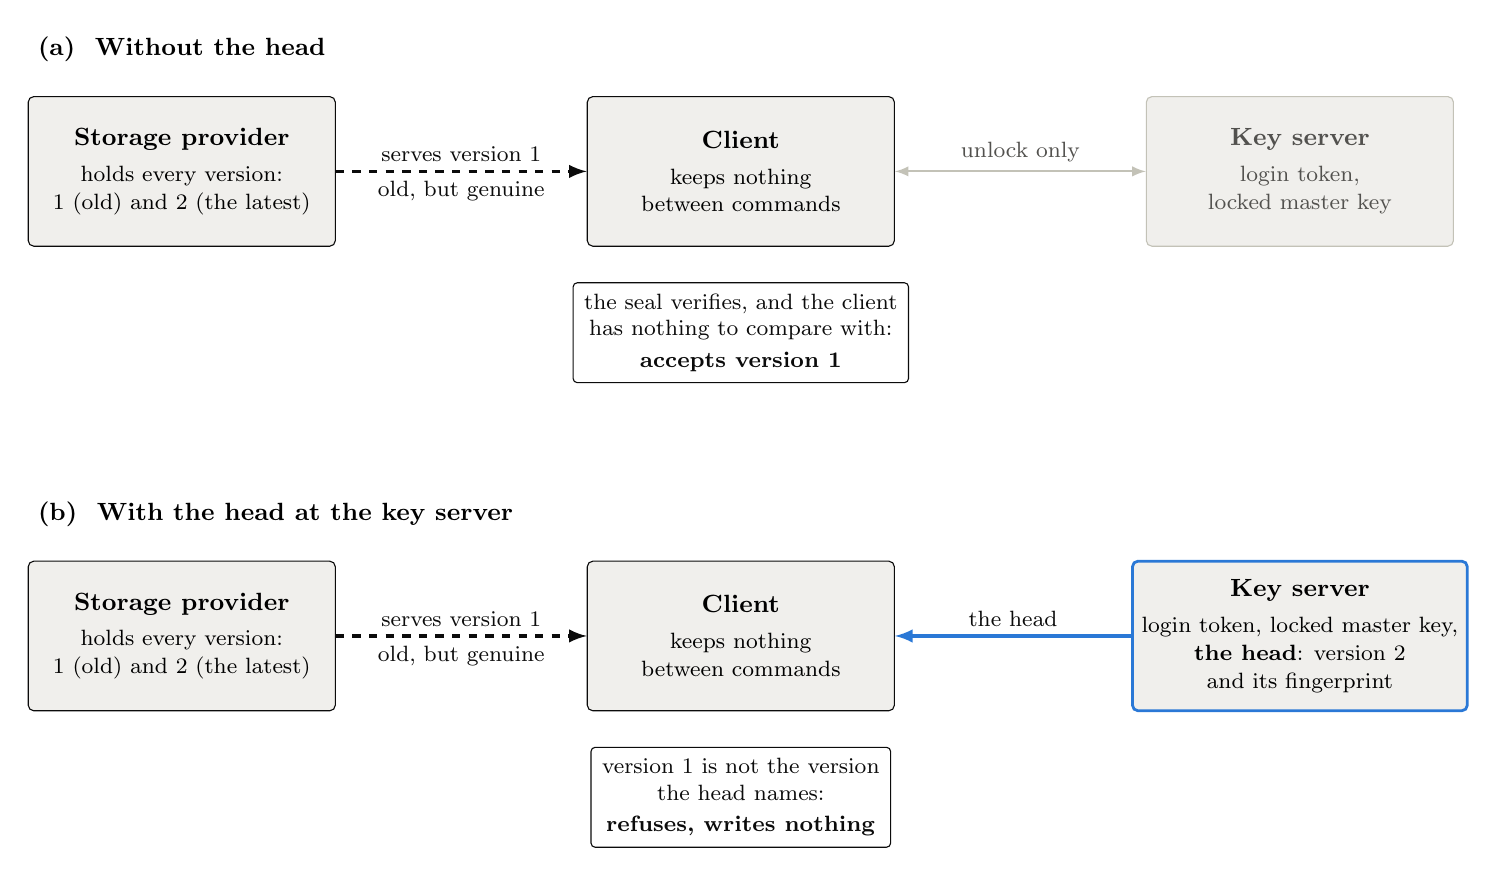
\begin{tikzpicture}
% ---------------------------------------------------------------- (a) without the head
\node[font=\small\bfseries, anchor=west] at (-1.95,1.55) {(a)\ \ Without the head};
\node[box] (Da) at (0,0)    {\textbf{Storage provider}\\[2pt]\footnotesize holds every version:\\[-1pt]\footnotesize 1 (old) and 2 (the latest)};
\node[box] (Ca) at (7.1,0)  {\textbf{Client}\\[2pt]\footnotesize keeps nothing\\[-1pt]\footnotesize between commands};
\node[box, quiet] (Ka) at (14.2,0) {\textbf{Key server}\\[2pt]\footnotesize login token,\\[-1pt]\footnotesize locked master key};
\draw[bad] (Da) -- node[lab, above] {serves version 1} node[lab, below] {old, but genuine} (Ca);
\draw[<->, draw=rule, line width=0.7pt] (Ca) -- node[lab, above, text=inktwo] {unlock only} (Ka);
\node[outcome, below=0.45cm of Ca] (oa) {the seal verifies, and the client\\ has nothing to compare with:\\[2pt] \textbf{accepts version 1}};
% ---------------------------------------------------------------- (b) with the head
\begin{scope}[yshift=-5.9cm]
\node[font=\small\bfseries, anchor=west] at (-1.95,1.55) {(b)\ \ With the head at the key server};
\node[box] (Db) at (0,0)    {\textbf{Storage provider}\\[2pt]\footnotesize holds every version:\\[-1pt]\footnotesize 1 (old) and 2 (the latest)};
\node[box] (Cb) at (7.1,0)  {\textbf{Client}\\[2pt]\footnotesize keeps nothing\\[-1pt]\footnotesize between commands};
\node[box, draw=head, line width=1.0pt] (Kb) at (14.2,0) {\textbf{Key server}\\[2pt]\footnotesize login token, locked master key,\\[-1pt]\footnotesize \textbf{the head}: version 2\\[-1pt]\footnotesize and its fingerprint};
\draw[bad] (Db) -- node[lab, above] {serves version 1} node[lab, below] {old, but genuine} (Cb);
\draw[hmsg] (Kb) -- node[lab, above] {the head} (Cb);
\node[outcome, below=0.45cm of Cb] (ob) {version 1 is not the version\\ the head names:\\[2pt] \textbf{refuses, writes nothing}};
\end{scope}
\end{tikzpicture}
\end{document}
